\section{基本不等式}

本节要点:
\begin{itemize}
    \item 掌握四类均值的概念;
    \item 深刻理解四类均值的实际意义;
    \item 深刻理解围绕它们的不等式。
\end{itemize}

~

教材只讨论了一个基本不等式
\[
a+b\geqslant 2\sqrt{ab}
\]
但我们进行扩展。

\begin{definition}
设实数$x_1,x_2,\cdots ,x_n\in \mathbb{R} $,称:
\begin{itemize}
    \item 它们的和与个数的比为{\bf 算数均值}(arithmetic mean),记作$A_n$;
    \item 它们各自的倒数的算数均值的倒数为{\bf 调和均值}(harmonic mean),也成为{\bf 倒数均值},记作$H_n$;
    \item 它们各自的平方的算数均值的算数平方根为{\bf 平方均值}(quadratic mean),也称为{\bf 均方根}(Root Mean Square,RMS),记作$Q_n$;
    \item 它们的乘积的$n$次算数平方根为{\bf 几何均值}(geometric mean),记作$G_n$。
\end{itemize}
\begin{align*}
&A_n=\frac{x_1+x_2+\cdots +x_n}{n}=\frac{\sum_{i=i}^n{x_i}}{n} \\
&H_n=\frac{n}{\frac{1}{x_1}+\frac{1}{x2}+\cdots \frac{1}{x_n}}=\frac{n}{\sum_{i=i}^n{\frac{1}{x_i}}} \\
&Q_n=\sqrt{\frac{x_{1}^{2}+x_{2}^{2}+\cdots +x_{n}^{2}}{n}}=\sqrt{\frac{\sum_{i=i}^n{x_{i}^{2}}}{n}} \\
&G_n=\sqrt[n]{x_1x_2\cdots x_n}
\end{align*}
\end{definition}

各类均值的产生是有其生产实践的背景的,目的是在一个目标总量下用均值代替各个分量,也即:
\[
\text{均值的和}=\text{各分量的和}=\text{目标总量}
\]

{\bf 算术均值}

算数均值非常直观,其目标总量就是直接累加,如平均成绩、平均每个人分到的苹果数等。

{\bf 调和均值}

调和均值的目标总量是倒数和,换个表述方式或许更易理解:
\[
\frac{1}{x_1}+\frac{1}{x_2}+\cdots \frac{1}{x_n}=\frac{n}{H_n}
\]
往往用于计算某些“率”,如已知并联电阻$R_1,R_2$求等效电阻,这里的目标总量就是流过两个支路的电流总和:
\[
\frac{U}{R_e}=\frac{U}{R_1}+\frac{U}{R_2} \quad \Rightarrow \quad \frac{1}{R_e}=\frac{1}{R_1}+\frac{1}{R_2}
\]
还如平均速度等,可自行推导。

{\bf 平方均值}

平方均值的目标总量在平方和,往往是跟能量相关,常用于计算交流电的平均电压、平均电流等。如为表征正弦电压的做功能力,我们可以定义电压的有效值为该周期性电压在电阻上一个周期内所作的相同的功,目标总量为总做功,即:
\[
\int_0^T{\frac{u^2\left( t \right)}{R}\cdot dt}=\frac{U^2}{R}\cdot T \quad \Rightarrow \quad U=\sqrt{\frac{1}{T}\cdot \int_0^T{\frac{u^2\left( t \right)}{R}\cdot dt}}
\]

{\bf 几何均值}

几何均值的目标总量为几何体的测度,如平面的面积、三维物体的体积,我们用等面积的正方形等效长方形,用等体积的正方体等效长方体等。

\begin{figure}[h]
\centering
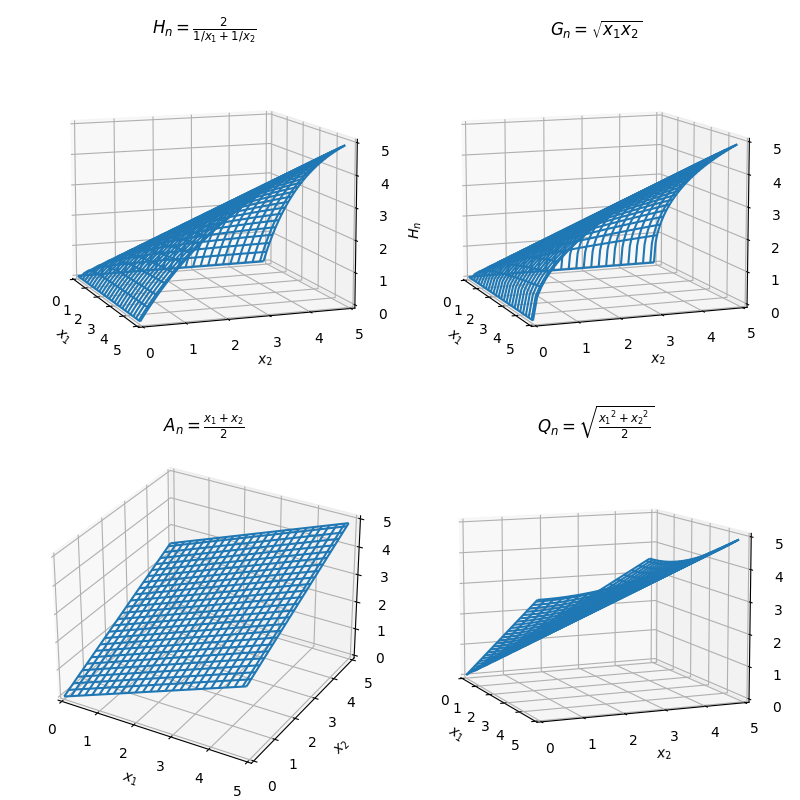
\includegraphics[height=9cm]{2.2-1.png}
\end{figure}

四类均值的图形如上,为方便作图我们只取两个变量,不难发现:
\begin{itemize}
    \item $H_n$和$G_n$弯向下,且$H_n$的下弯速度大于$G_n$;
    \item $A_n$是一个平面,必然大于$H_n$和$G_n$;
    \item $Q_n$弯向上,必然大于$A_n$;
    \item $x_1=x_2$为它们公共的交线。
\end{itemize}

\begin{theorem}[均值不等式定理]
设实数$x_1,x_2,\cdots ,x_n\in \mathbb{R} $,则四类均值有:
\[
H_n\leqslant G_n\leqslant A_n\leqslant Q_n
\]
或写成:
\[
\frac{n}{\sum_{i=i}^n{\frac{1}{x_i}}}\leqslant \sqrt[n]{x_1x_2\cdots x_n}\leqslant \frac{\sum_{i=i}^n{x_i}}{n}\leqslant \sqrt{\frac{\sum_{i=i}^n{x_{i}^{2}}}{n}}
\]
当且仅当$x_1=x_2=\cdots =x_n$时等号成立。
\end{theorem}

\begin{proof}
构造直角三角形$\bigtriangleup ABC$,如图,令$AB=\frac{x_1+x_2}{2},AC=\frac{x_1-x_2}{2}$,由勾股定理可得$BC=\sqrt{\frac{{x_1}^2+{x_2}^2}{2}}$,可见:
\[
\frac{x_1+x_2}{2}\leqslant \sqrt{\frac{{x_1}^2+{x_2}^2}{2}}
\]

\begin{figure}[h]
\centering
\begin{tikzpicture}[line join=round, scale=1]
\coordinate[label=above:{$A$}] (A) at (0,0);
\coordinate[label=above:{$C$}] (C) at (-2,0);
\coordinate[label=below:{$B$}] (B) at (0,-4);
\coordinate[label=above:{$E$}] (E) at (1.732,0);
\coordinate[label=below:{$D$}] (D) at (1.732,-3);
\coordinate[label=above:      {$\frac{x_1-x_2}{2}$}]                    (ac) at ($(A)!0.5!(C)$);
\coordinate[label=left:       {$\sqrt{\frac{x_{1}^{2}+x_{2}^{2}}{2}}$}] (bc) at ($(C)!0.5!(B)$);
\coordinate[label=above left: {$\frac{x_1+x_2}{2}$}]                    (ab) at ($(A)!0.5!(B)$);
\coordinate[label=below:      {$\sqrt{x_1x_2}$}]                        (ad) at ($(A)!0.5!(D)$);
\coordinate[label=below right:{$\frac{x_1-x_2}{2}$}]                    (bd) at ($(B)!0.5!(D)$);
\coordinate[label=right:      {$\frac{2x_1x_2}{x_1+x_2}$}]              (de) at ($(D)!0.5!(E)$);
\draw[thick] (C)--(E)--(D)--(B)--(C) (B)--(A)--(D);
\pic["$\theta $",draw,angle radius=0.5cm,angle eccentricity=1.5] {angle=B--A--D};
\pic["$\theta $",draw,angle radius=0.5cm,angle eccentricity=1.5] {angle=E--D--A};
\end{tikzpicture}
\end{figure}

再以$AB$为斜边构造直角三角形$\bigtriangleup ABD$,令$BD=AC=\frac{x_1-x_2}{2}$,由勾股定理可得$AD=\sqrt{x_1x_2}$,可见:
\[
\sqrt{x_1x_2}\leqslant \frac{x_1+x_2}{2}
\]

继续作直角三角形$\bigtriangleup ADE$,令$ED\parallel AB$,于是$\angle BAD=\angle ADE=\theta $,则有:
\begin{align*}
&\because \cos \theta =\frac{AD}{AB}=\frac{ED}{AD} \\
&\therefore ED=\frac{AD^2}{AB}=\frac{x_1x_2}{\frac{x_1+x_2}{2}}=\frac{2x_1x_2}{x_1+x_2}=\frac{2}{\frac{1}{x_1}+\frac{1}{x_2}} \\
&\therefore \frac{2}{\frac{1}{x_1}+\frac{1}{x_2}}\leqslant \sqrt{x_1x_2}
\end{align*}
\end{proof}

\begin{proof}
使用向量的方法证明
\[
\frac{x_1+x_2}{2}\leqslant \sqrt{\frac{{x_1}^2+{x_2}^2}{2}}
\]
化简如下:
\[
\frac{x_1\cdot \frac{\sqrt{2}}{2}+x_2\cdot \frac{\sqrt{2}}{2}}{\sqrt{{x_1}^2+{x_2}^2}}\leqslant 1
\]
于是就可以发现,分子是两个向量的内积,分母是向量的模,整个表达式就是两个向量夹角的余弦,于是可设$\boldsymbol{a}=\left( x_1,x_2 \right) ,\boldsymbol{b}=\left( \frac{\sqrt{2}}{2},\frac{\sqrt{2}}{2} \right) $,得到:
\[
\cos \theta =\frac{\boldsymbol{a}\cdot \boldsymbol{b}}{\left| \boldsymbol{a} \right|\left| \boldsymbol{b} \right|}=\frac{x_1\cdot \frac{\sqrt{2}}{2}+x_2\cdot \frac{\sqrt{2}}{2}}{\sqrt{{x_1}^2+{x_2}^2}}\leqslant 1
\]
\end{proof}

~

\begin{example}[综合运用4,难度:$\star $]
已知$x,y,z$都是整数,求证
\[
\left( x+y \right) \left( y+z \right) \left( z+x \right) \geqslant 8xyz
\]
\end{example}

解:

\begin{align*}
&\quad \left( x+y \right) \left( y+z \right) \left( z+x \right) \\
&=\left( xy+xz+y^2+yz \right) \left( z+x \right) \\
&=xyz+x^2y+xz^2+x^2z+y^2z+y^2x+yz^2+xyz
\end{align*}
观察分析:
\begin{align*}
&x^2y+yz^2\geqslant 2y\sqrt{x^2z^2}=2xyz \\
&xz^2+y^2x\geqslant 2x\sqrt{z^2y^2}=2xyz \\
&x^2z+y^2z\geqslant 2z\sqrt{x^2y^2}=2xyz
\end{align*}
略,证毕。

\begin{tcolorbox}
本题只需尝试将左边展开即可发现方法。
\end{tcolorbox}

~

\begin{example}[拓广探索7,难度:$\star \star $]
一家商店使用一架两臂不等长的天平秤黄金,一位顾客到商店购买10g黄金,售货员先将5g的砝码放在天平左盘中,取出一些黄金放在天平右盘中使天平平衡;再将5g的砝码放在天平的右盘中,再取出一些黄金放在天平左盘中使天平平衡;最后将两次称得的黄金交给顾客。你认为顾客购得的黄金是小于10g,等于10g,还是大于10g?为什么?
\end{example}

解:

这个问题较为复杂,我们可以先尝试用一些数学式子描述该问题。假设天平左右两个臂的臂长分别为$l_L,l_R$,则根据力矩相等易得两次称重黄金的数学表示为:
\begin{align*}
&5\cdot l_L=A\cdot l_R \\
&B\cdot l_L=5\cdot l_R
\end{align*}
稍稍化简得:
\begin{align*}
&A=5\cdot \frac{l_L}{l_R} \\
&B=5\cdot \frac{l_R}{l_L}
\end{align*}
易得:
\[
A+B\geqslant 2\sqrt{5\cdot \frac{l_L}{l_R}\cdot 5\cdot \frac{l_R}{l_L}}=10
\]

\begin{tcolorbox}
本题关键在于获得$A,B$的表达式,一旦获得了,不难发现其互为倒数的关系,也就能自然想到基本不等式了。
\end{tcolorbox}

~

\begin{example}[拓广探索8,难度:$\star \star $]
设矩形$ABCD$($AB>AD$)的周长为24cm,把$\bigtriangleup ABC$沿$AC$向$\bigtriangleup ADC$折叠,$AB$折过去后交$DC$于点$P$。
设$AB=x\mathrm{cm}$,求$\bigtriangleup ADP$的最大面积及相应$x$的值。
\end{example}

\begin{figure}[h]
\centering
\begin{tikzpicture}[line join=round, scale=0.75]
\coordinate[label=above left: {$A$}]  (A)  at (-2.5,1);
\coordinate[label=above right:{$B$}]  (B)  at (2.5,1);
\coordinate[label=below right:{$C$}]  (C)  at (2.5,-1);
\coordinate[label=below left: {$D$}]  (D)  at (-2.5,-1);
\draw[thick] (D)--(A)--(B)--(C) (A)--(C);
\coordinate                     (tb) at ($(A)!(B)!(C)$);
\coordinate[label=below:{$B'$}] (B') at ($(B)!2.0!(tb)$);
\draw[thick,name path=l1] (D)--(C);
\draw[thick,blue,name path=l2] (A)--(B');
\path [name intersections={of=l1 and l2}] coordinate[label=below left:$P$] (P) at (intersection-1);
\draw[thick,blue] (B')--(C);
\coordinate                           (tp) at ($(A)!(P)!(C)$);
\coordinate[label=above right:{$P'$}] (P') at ($(P)!2.0!(tp)$);
\draw[thick,dashed,red] (P)--(P')--(C);
\coordinate[label=above:{$x$}]    (x)  at ($(A)!0.5!(B)$);
\coordinate[label=left: {$12-x$}] (x') at ($(A)!0.5!(D)$);
\coordinate[label=below:{$y$}]    (y)  at ($(D)!0.5!(P)$);
\end{tikzpicture}
\end{figure}

解:

令$DP$长$y$,则$\bigtriangleup ADP$的面积为:
\[
S_{\bigtriangleup ADP}=\frac{1}{2}\left( 12-x \right) y
\]
不难证明$\bigtriangleup ADP,\bigtriangleup CB'P$均为直角三角形,且全等,于是
\begin{align*}
&\because PC=PA=\sqrt{\left( 12-x \right) ^2+y^2} \\
&\therefore x=\sqrt{\left( 12-x \right) ^2+y^2}+y \\
&\therefore y=\frac{12x-72}{x}
\end{align*}
带入面积消去$y$,得:
\begin{align*}
S_{\bigtriangleup ADP}&=\frac{1}{2}\left( 12-x \right) y=\frac{1}{2}\left( 12-x \right) \frac{12x-72}{x} \\
&=6\cdot \frac{-x^2+18x-72}{x} \\
&=6\cdot \left( -x-\frac{72}{x}+18 \right)
\end{align*}
其中,$x+\frac{72}{x}\geqslant 2\sqrt{72}=12\sqrt{2}$,当且仅当$x=\frac{72}{x},x=\sqrt{72}$时等号成立,于是:
\[
S_{\bigtriangleup ADP}\leqslant 6\cdot \left( 18-12\sqrt{2} \right)
\]

\begin{tcolorbox}
本题的关键在于获得$S_{\bigtriangleup ADP}$的表达式和$x,y$的约束关系。一旦获得了,接下去就是化简和基本不等式。
\end{tcolorbox}

\begin{tcolorbox}
高中阶段的求解最值问题,最终都会转化为求解
\[
\left( Ax \right) +\left( \frac{B}{x} \right) \quad \text{或} \quad \left( Ax \right) \cdot \left( \frac{B}{x} \right)
\]
的最值问题,也即基本不等式。关键在于理解问题和观察图形,将实际问题或几何图形建模成代数问题。上面两题很有典型性,一题是实际应用题,另一题是几何题。结合上一章的说到的数学范式,认真思考上面两题,总结你的解题范式,XML。
\end{tcolorbox}




